\documentclass[../DoAn.tex]{subfiles}
\begin{document}
Phần này khảo sát nhu cầu của người mua hàng, nhu cầu của cửa hàng nội thất nhỏ và vừa, đồng thời xem xét một số giải pháp liên quan trong nước và trên thế giới. Mục tiêu là xác định các chức năng đã được hỗ trợ, các điểm còn hạn chế và khoảng trống mà hệ thống đề xuất cần giải quyết.
 
\section{Khảo sát hiện trạng}
\label{section:2.1}

Phần này khảo sát nhu cầu của người mua hàng, nhu cầu của cửa hàng nội thất nhỏ và vừa, đồng thời xem xét một số nhóm giải pháp liên quan trong nước và trên thế giới. Mục tiêu của phần khảo sát là xác định những chức năng đã được các hệ thống hiện có hỗ trợ, những điểm còn hạn chế và khoảng trống mà hệ thống đề xuất cần giải quyết.

\subsection{Nhu cầu của người mua hàng nội thất}
\label{subsection:2.1.1}

Đối với người mua hàng nội thất, nhu cầu thường không chỉ là tìm một sản phẩm theo tên hoặc theo khoảng giá. Người dùng thường cần được tư vấn theo bối cảnh sử dụng cụ thể, chẳng hạn như chọn bàn làm việc cho phòng nhỏ, chọn ghế sofa phù hợp với phòng khách hiện đại hoặc tìm tủ có kích thước phù hợp với không gian đang có.

Quá trình lựa chọn sản phẩm cũng thường diễn ra qua nhiều lượt trao đổi. Ban đầu, người dùng có thể chỉ nêu một nhu cầu chung, sau đó thay đổi ngân sách, điều chỉnh loại sản phẩm, yêu cầu phong cách khác hoặc muốn so sánh thêm một số lựa chọn. Vì vậy, hệ thống tư vấn cần ghi nhận được ngữ cảnh hội thoại và điều chỉnh gợi ý theo thay đổi của người dùng.

Bên cạnh tư vấn, người mua còn cần so sánh sản phẩm và tham khảo giá trước khi quyết định. Với sản phẩm nội thất, việc so sánh cần xét nhiều yếu tố như giá, chất liệu, kích thước, kiểu dáng, phong cách và cửa hàng cung cấp. Do đó, hệ thống cần hỗ trợ người dùng tiếp cận thông tin nhanh hơn, so sánh rõ ràng hơn và có thêm cơ sở khi đánh giá mức giá của sản phẩm.
\subsection{Nhu cầu của cửa hàng nội thất nhỏ và vừa}
\label{subsection:2.1.2}

Đối với các cửa hàng nội thất nhỏ và vừa, nhu cầu chính là có một công cụ hỗ trợ tư vấn khách hàng dựa trên dữ liệu sản phẩm của chính cửa hàng. Dữ liệu sản phẩm nội thất thường gồm nhiều thuộc tính như tên sản phẩm, mô tả, giá, chất liệu, kích thước, loại sản phẩm, phong cách và đường dẫn sản phẩm. Khi số lượng sản phẩm tăng hoặc dữ liệu thay đổi, việc tư vấn thủ công dễ thiếu nhất quán, phụ thuộc vào nhân viên và khó mở rộng trên nhiều kênh.

Ngoài tư vấn, cửa hàng còn cần quản lý quá trình vận hành chatbot, gồm cập nhật dữ liệu sản phẩm, quản lý nguồn dữ liệu dùng để xây dựng knowledge base, theo dõi trạng thái xử lý dữ liệu, xem lịch sử hội thoại, ghi nhận khách hàng tiềm năng và tiếp nhận yêu cầu mua hàng phát sinh từ hội thoại.

Một yêu cầu quan trọng khác là hệ thống phải phù hợp với môi trường nhiều cửa hàng. Mỗi cửa hàng cần có dữ liệu sản phẩm, chatbot, cấu hình và lịch sử hội thoại riêng, nhưng vẫn có thể dùng chung một nền tảng. Vì vậy, hệ thống cần hỗ trợ mô hình multi-tenant để tách biệt dữ liệu giữa các cửa hàng và giảm chi phí triển khai so với việc mỗi cửa hàng tự xây dựng một chatbot AI riêng.

\subsection{Khảo sát một số nhóm giải pháp hiện có}
\label{subsection:2.1.3}
Hiện nay, các giải pháp liên quan đến bài toán của đề tài có thể chia thành một số nhóm chính: website bán hàng nội thất, nền tảng thương mại điện tử, chatbot kịch bản/marketing, live chat và chatbot chăm sóc khách hàng, và AI agent có sử dụng knowledge base. Để khảo sát cụ thể hơn, phần này xem xét một số hệ thống tiêu biểu như JYSK Việt Nam\footnote{JYSK Việt Nam, \textit{Trang chủ JYSK Việt Nam}, \url{https://jysk.vn/}, truy cập lần cuối ngày 29/05/2026}, IKEA Kreativ\footnote{IKEA, \textit{IKEA Kreativ / Home Design}, \url{https://www.ikea.com/us/en/home-design/}, truy cập lần cuối ngày 29/05/2026}, ManyChat\footnote{ManyChat, \textit{ManyChat Platform}, \url{https://manychat.com/}, truy cập lần cuối ngày 29/05/2026}, Tidio\footnote{Tidio, \textit{Tidio Customer Service Platform}, \url{https://www.tidio.com/}, truy cập lần cuối ngày 29/05/2026} và Intercom Fin\footnote{Intercom, \textit{Fin AI Agent explained}, \url{https://www.intercom.com/help/en/articles/7120684-fin-ai-agent-explained}, truy cập lần cuối ngày 29/05/2026}.

Ở Việt Nam, các website bán hàng nội thất như JYSK Việt Nam cung cấp danh mục sản phẩm, thông tin mô tả, hình ảnh, giá bán và các nhóm sản phẩm phục vụ nhu cầu tra cứu trực tuyến của khách hàng. Nhóm giải pháp này phù hợp với nhu cầu xem và tìm sản phẩm, nhưng người dùng vẫn phải tự đọc thông tin, tự lọc và tự so sánh giữa các lựa chọn. Các chức năng tư vấn bằng ngôn ngữ tự nhiên, ghi nhớ ngữ cảnh hội thoại hoặc tham chiếu giá theo nhu cầu cụ thể thường chưa phải trọng tâm của nhóm hệ thống này.

Trên thế giới, IKEA là một ví dụ tiêu biểu cho hướng kết hợp dữ liệu sản phẩm với trải nghiệm hỗ trợ mua sắm và thiết kế không gian. Công cụ IKEA Kreativ cho phép người dùng thử sản phẩm trong phòng ảo hoặc trong không gian của chính mình, từ đó hỗ trợ quá trình hình dung và lựa chọn sản phẩm nội thất. Ngoài ra, IKEA cũng đã giới thiệu trải nghiệm trợ lý AI\footnote{Ingka Group, \textit{IKEA launches new AI-powered assistant in OpenAI GPT Store}, \url{https://www.ingka.com/newsroom/ikea-launches-new-ai-powered-assistant-in-openai-gpt-store/}, truy cập lần cuối ngày 29/05/2026} nhằm hỗ trợ người dùng tìm cảm hứng thiết kế và lựa chọn sản phẩm phù hợp hơn. Tuy nhiên, các giải pháp này chủ yếu phục vụ hệ sinh thái bán lẻ riêng của một thương hiệu lớn, chưa trực tiếp giải quyết bài toán một nền tảng dùng chung cho nhiều cửa hàng nhỏ và vừa, trong đó mỗi cửa hàng có dữ liệu sản phẩm và chatbot riêng.

Đối với nhóm chatbot kịch bản và chatbot marketing, ManyChat là một nền tảng tiêu biểu. ManyChat hỗ trợ tự động hóa hội thoại trên các kênh như Instagram, Facebook Messenger và SMS, giúp doanh nghiệp phản hồi tin nhắn, tương tác với khách hàng và hỗ trợ hoạt động bán hàng theo các luồng được thiết kế sẵn. Ưu điểm của nhóm giải pháp này là dễ triển khai và phù hợp với các kịch bản marketing phổ biến. Tuy nhiên, khi khách hàng thay đổi nhu cầu, hỏi nhiều lượt hoặc cần so sánh sản phẩm dựa trên dữ liệu chi tiết, chatbot dạng kịch bản thường bị hạn chế về khả năng hiểu ngữ cảnh và đưa ra tư vấn linh hoạt.

Với nhóm live chat và chatbot chăm sóc khách hàng, Tidio là một ví dụ phổ biến. Nền tảng này cung cấp live chat, helpdesk, chatbot/AI agent và các chức năng hỗ trợ tạo khách hàng tiềm năng. Nhóm giải pháp này mạnh ở việc quản lý hội thoại, phản hồi khách hàng và hỗ trợ nhân viên chăm sóc khách hàng. Tuy nhiên, trọng tâm của các nền tảng này thường là hỗ trợ khách hàng nói chung, chưa chuyên biệt cho bài toán tư vấn sản phẩm nội thất dựa trên knowledge base riêng của từng cửa hàng, so sánh sản phẩm và tham chiếu giá.

Gần với hướng tiếp cận RAG hơn là các AI agent có sử dụng dữ liệu doanh nghiệp, tiêu biểu như Intercom Fin\footnote{Intercom, \textit{Add your content for Fin AI Agent}, \url{https://www.intercom.com/help/en/articles/7837514-add-your-content-for-fin-ai-agent}, truy cập lần cuối ngày 29/05/2026}. Intercom giới thiệu Fin như một AI agent phục vụ chăm sóc khách hàng, có thể được tích hợp trong hệ thống helpdesk và sử dụng nội dung hỗ trợ do doanh nghiệp cung cấp để tạo câu trả lời. Nhóm giải pháp này cho thấy khả năng ứng dụng AI để trả lời dựa trên dữ liệu riêng của tổ chức. Tuy nhiên, đây vẫn là nền tảng tổng quát cho chăm sóc khách hàng, không tập trung riêng vào bài toán multi-tenant cho cửa hàng nội thất, cũng không mặc định hỗ trợ các chức năng đặc thù như so sánh sản phẩm nội thất và tham chiếu giá theo dữ liệu tổng hợp từ nhiều cửa hàng.

\subsection{So sánh các giải pháp theo tiêu chí của đề tài}
\label{subsection:2.1.4}

Để làm rõ khoảng trống của các giải pháp hiện có, Bảng~\ref{table:compare-related-solutions} so sánh một số nhóm giải pháp theo các tiêu chí bám sát mục tiêu của đề tài. Do các hệ thống thương mại không phải lúc nào cũng công bố độ chính xác định lượng hoặc chi tiết kỹ thuật bên trong, bảng so sánh sử dụng mức đánh giá chức năng gồm: Có, Một phần, Không và Không rõ. Các chỉ số định lượng như độ chính xác truy xuất, độ trễ phản hồi, chất lượng câu trả lời và khả năng hoàn thành tác vụ hội thoại sẽ được đánh giá chi tiết ở chương thực nghiệm.

\begin{table}[H]
\centering
\caption{So sánh tổng quan chức năng của các giải pháp hiện hành}
\label{table:compare-related-solutions}
\resizebox{\textwidth}{!}{
\begin{tabular}{|p{4.6cm}|p{2.3cm}|p{2.5cm}|p{2.2cm}|p{2.2cm}|p{2.3cm}|}
\hline
\textbf{Tiêu chí} &
\textbf{JYSK Việt Nam} &
\textbf{IKEA\newline(Kreativ/AI Assistant)} &
\textbf{ManyChat} &
\textbf{Tidio} &
\textbf{Intercom Fin} \\
\hline
Tra cứu và xem thông tin sản phẩm & Có & Có & Một phần & Một phần & Một phần \\
\hline
Tư vấn sản phẩm bằng ngôn ngữ tự nhiên & Không / Hạn chế & Một phần & Một phần & Có & Có \\
\hline
Hội thoại nhiều lượt theo ngữ cảnh & Không & Một phần & Hạn chế & Một phần & Có \\
\hline
Khai thác dữ liệu riêng / knowledge base & Hạn chế & Một phần & Hạn chế & Một phần & Có \\
\hline
Hỗ trợ nhiều cửa hàng / tách biệt dữ liệu & Không & Không & Tùy nền tảng & Tùy nền tảng & Tùy nền tảng \\
\hline
So sánh sản phẩm theo nhiều tiêu chí & Một phần & Một phần & Hạn chế & Hạn chế & Tùy nền tảng \\
\hline
Tham chiếu giá sản phẩm & Một phần & Một phần & Không & Hạn chế & Tùy nền tảng \\
\hline
Tạo lead hoặc yêu cầu mua hàng từ hội thoại & Một phần & Một phần & Có & Có & Có \\
\hline
Mức độ phù hợp với cửa hàng nội thất nhỏ và vừa & Một phần & Hạn chế & Một phần & Một phần & Một phần \\
\hline
\end{tabular}
}
\end{table}

Từ bảng so sánh có thể thấy mỗi giải pháp hiện hành chỉ đáp ứng tốt một phần của bài toán. JYSK Việt Nam và IKEA mạnh về hiển thị, tra cứu và hỗ trợ lựa chọn sản phẩm, nhưng chưa tập trung vào tư vấn hội thoại nhiều lượt cho nhiều cửa hàng độc lập. ManyChat và Tidio mạnh về tự động hóa hội thoại, chăm sóc khách hàng và tạo khách hàng tiềm năng, nhưng còn hạn chế khi cần tư vấn dựa trên dữ liệu sản phẩm chi tiết, so sánh sản phẩm và tham chiếu giá. Intercom Fin gần hơn với hướng sử dụng AI và knowledge base, nhưng vẫn là một nền tảng tổng quát, chưa chuyên biệt cho bài toán tư vấn bán hàng nội thất theo mô hình multi-tenant.

Vì vậy, khoảng trống của các giải pháp hiện hành là chưa có một hệ thống tập trung vào cửa hàng nội thất nhỏ và vừa, vừa hỗ trợ dữ liệu riêng theo từng cửa hàng, vừa hỗ trợ hội thoại nhiều lượt, so sánh sản phẩm và tham chiếu giá trên cùng một nền tảng.

\section{Tổng quan chức năng}
\label{section:2.2}

Dựa trên kết quả khảo sát hiện trạng ở phần \ref{section:2.1}, hệ thống được xây dựng để hỗ trợ các nhóm chức năng chính của một nền tảng chatbot RAG cho nhiều cửa hàng nội thất. Các chức năng trọng tâm gồm tư vấn sản phẩm theo cửa hàng, tư vấn tổng quát, tham chiếu giá sản phẩm, tạo yêu cầu mua hàng, quản lý chatbot, quản lý knowledge base, quản lý hội thoại, quản lý lead, quản lý yêu cầu mua hàng, quản lý tenant và quản lý thành viên cửa hàng.

Hệ thống có bốn nhóm tác nhân chính: người dùng cuối, nhân viên cửa hàng, quản trị cửa hàng và quản trị hệ thống. Ngoài ra, hệ thống sử dụng Claude Sonnet để hỗ trợ xử lý ngôn ngữ tự nhiên và sinh câu trả lời tư vấn. Các use case và quy trình nghiệp vụ quan trọng được trình bày trong phần này, làm cơ sở cho phần đặc tả chức năng ở mục \ref{section:2.3}.

\subsection{Biểu đồ use case tổng quát}
\label{subsection:2.2.1}

Biểu đồ use case tổng quát của hệ thống được trình bày trong Hình~\ref{fig:usecase-tong-quat}. Biểu đồ thể hiện phạm vi chức năng chính của hệ thống, các tác nhân tham gia và mối liên hệ giữa hệ thống với Claude Sonnet.

\begin{figure}[H]
    \centering
    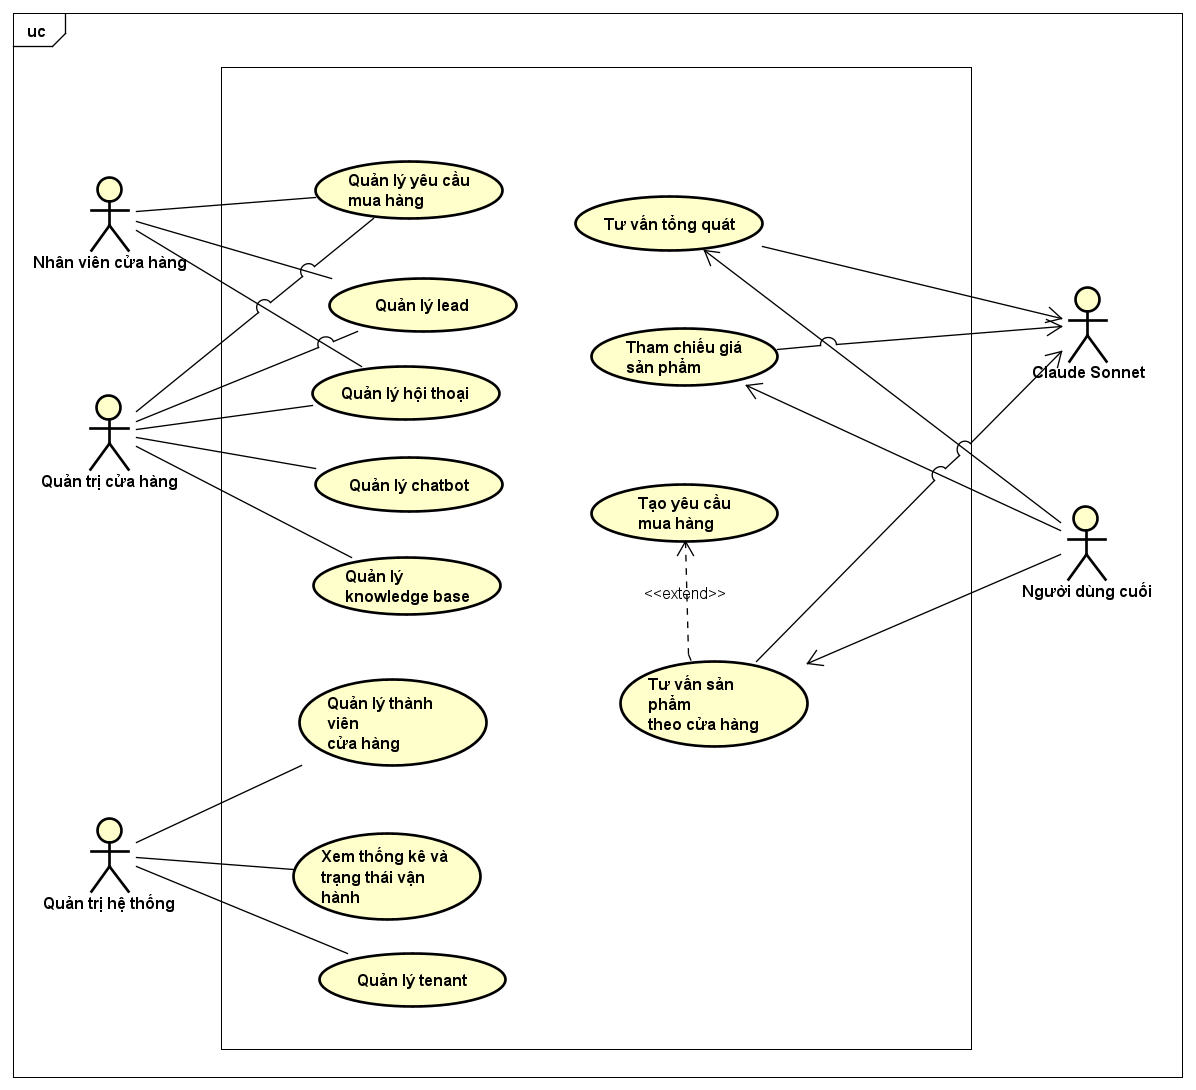
\includegraphics[width=0.95\textwidth]{../Hinhve/Hinh2_1_usecase_tong_quat.png}
    \caption{Biểu đồ use case tổng quát của hệ thống}
    \label{fig:usecase-tong-quat}
\end{figure}

Người dùng cuối tương tác với chatbot để được tư vấn sản phẩm theo cửa hàng, tư vấn tổng quát, tham chiếu giá sản phẩm và tạo yêu cầu mua hàng. Đây là nhóm chức năng trực tiếp phục vụ mục tiêu hỗ trợ tư vấn bán hàng trong đề tài.

Nhân viên cửa hàng xử lý các thông tin phát sinh sau quá trình tư vấn, gồm quản lý hội thoại, quản lý lead và quản lý yêu cầu mua hàng. Tác nhân này tập trung vào việc theo dõi nhu cầu của khách hàng, phản hồi lead, nhận xử lý yêu cầu mua hàng và cập nhật trạng thái xử lý.

Quản trị cửa hàng vận hành các chức năng trong phạm vi tenant của mình. Các chức năng chính gồm quản lý chatbot, quản lý knowledge base, quản lý hội thoại, quản lý lead và quản lý yêu cầu mua hàng. Nhóm chức năng này giúp cửa hàng chủ động cấu hình chatbot, cập nhật nguồn dữ liệu và theo dõi hoạt động tư vấn.

Quản trị hệ thống quản lý các thành phần chung của nền tảng, gồm quản lý tenant, quản lý thành viên cửa hàng, xem thống kê và trạng thái vận hành. Nhóm chức năng này phục vụ yêu cầu multi-tenant, trong đó nhiều cửa hàng cùng sử dụng một hệ thống nhưng dữ liệu, cấu hình và quyền truy cập được tách biệt.

Claude Sonnet là tác nhân ngoài hệ thống. AI Service gửi yêu cầu đến Claude Sonnet trong các chức năng cần sinh câu trả lời bằng ngôn ngữ tự nhiên, đặc biệt là tư vấn tổng quát, tư vấn sản phẩm theo cửa hàng và tham chiếu giá sản phẩm.

\subsection{Biểu đồ use case phân rã Quản lý chatbot và knowledge base}
\label{subsection:2.2.2}

Biểu đồ use case phân rã nhóm chức năng quản lý chatbot và knowledge base được trình bày trong Hình~\ref{fig:usecase-quan-ly-chatbot-kb}. Nhóm chức năng này dành chủ yếu cho quản trị cửa hàng, phục vụ quá trình chuẩn bị dữ liệu và vận hành chatbot trong phạm vi từng tenant.

\begin{figure}[H]
    \centering
    
\includegraphics[width=0.95\textwidth]{../Hinhve/Hinh2_3_usecase_quan_ly_chatbot_kb.png}
    \caption{Biểu đồ use case phân rã Quản lý chatbot và knowledge base}
    \label{fig:usecase-quan-ly-chatbot-kb}
\end{figure}

Đối với chatbot, quản trị cửa hàng có thể tạo chatbot, xem danh sách chatbot và cập nhật cấu hình chatbot. Các chức năng này cho phép cửa hàng thiết lập chatbot phù hợp với mục đích tư vấn, dữ liệu sử dụng và cách phản hồi mong muốn.

Đối với knowledge base, quản trị cửa hàng có thể xem danh sách nguồn dữ liệu, thêm nguồn dữ liệu vào knowledge base, xóa nguồn dữ liệu khỏi knowledge base, rebuild knowledge base, xem trạng thái knowledge base và xem lịch sử rebuild. Đây là nhóm chức năng quan trọng vì chất lượng tư vấn của chatbot phụ thuộc trực tiếp vào dữ liệu được đưa vào knowledge base.

Quản trị hệ thống có thể theo dõi trạng thái knowledge base của các tenant ở mức tổng quan. Chức năng này giúp quản trị hệ thống nắm được tình trạng xử lý dữ liệu và hỗ trợ vận hành nền tảng.

\subsection{Biểu đồ use case phân rã Quản lý hội thoại, lead và yêu cầu mua hàng}
\label{subsection:2.2.3}

Biểu đồ use case phân rã nhóm chức năng quản lý hội thoại, lead và yêu cầu mua hàng được trình bày trong Hình~\ref{fig:usecase-quan-ly-hoi-thoai-yeu-cau}. Nhóm chức năng này dành cho nhân viên cửa hàng và quản trị cửa hàng sau khi người dùng đã tương tác với chatbot.

\begin{figure}[H]
    \centering
    
\includegraphics[width=0.95\textwidth]{../Hinhve/Hinh2_4_usecase_quan_ly_hoi_thoai_yeu_cau.png}
    \caption{Biểu đồ use case phân rã Quản lý hội thoại, lead và yêu cầu mua hàng}
    \label{fig:usecase-quan-ly-hoi-thoai-yeu-cau}
\end{figure}

Đối với hội thoại, nhân viên cửa hàng và quản trị cửa hàng có thể xem danh sách hội thoại, lọc hội thoại và xem chi tiết hội thoại. Các chức năng này giúp cửa hàng nắm được nhu cầu, nội dung trao đổi và các sản phẩm đã được chatbot tư vấn cho khách hàng.

Đối với lead, người dùng trong cửa hàng có thể xem danh sách lead, xem chi tiết lead, phản hồi lead qua kênh chat và cập nhật trạng thái lead. Các chức năng này giúp cửa hàng tiếp tục chăm sóc những khách hàng đã để lại nhu cầu hoặc thông tin liên hệ sau phiên tư vấn.

Đối với yêu cầu mua hàng, nhân viên cửa hàng có thể xem danh sách yêu cầu, lọc theo trạng thái, xem chi tiết, nhận xử lý và cập nhật trạng thái yêu cầu. Quản trị cửa hàng có thêm quyền phân công lại yêu cầu mua hàng cho nhân viên khác trong cùng tenant. Nhóm chức năng này liên kết trực tiếp với quá trình tư vấn, vì một phiên hội thoại có thể phát sinh lead hoặc yêu cầu mua hàng.

\subsection{Quy trình nghiệp vụ}
\label{subsection:2.2.4}

Bên cạnh các use case, hệ thống có ba quy trình nghiệp vụ chính: cấu hình chatbot và xây dựng knowledge base, chat tư vấn và tạo yêu cầu mua hàng, xử lý lead/yêu cầu mua hàng. Các quy trình này mô tả cách các chức năng được sử dụng nối tiếp nhau trong thực tế.

\subsubsection{Quy trình cửa hàng cấu hình chatbot và xây dựng knowledge base}
\label{subsubsection:2.2.4.1}

Quy trình cửa hàng cấu hình chatbot và xây dựng knowledge base được trình bày trong Hình~\ref{fig:activity-cau-hinh-chatbot-kb}. Quy trình bắt đầu từ quản trị cửa hàng và kết thúc khi quản trị cửa hàng xem được trạng thái xử lý của knowledge base.

\begin{figure}[H]
    \centering
    
\includegraphics[width=0.95\textwidth]{../Hinhve/Hinh2_6_activity_cau_hinh_chatbot_kb.png}
    \caption{Biểu đồ hoạt động quy trình cửa hàng cấu hình chatbot và xây dựng knowledge base}
    \label{fig:activity-cau-hinh-chatbot-kb}
\end{figure}

Quản trị cửa hàng đăng nhập vào hệ thống, truy cập trang quản lý chatbot, tạo hoặc cập nhật cấu hình chatbot. Sau đó, quản trị cửa hàng chuyển sang trang quản lý knowledge base, thêm hoặc cập nhật nguồn dữ liệu và kích hoạt rebuild knowledge base. Hệ thống xác thực thông tin đăng nhập, xử lý dữ liệu, rebuild knowledge base và cập nhật trạng thái xử lý. Quản trị cửa hàng xem lỗi, lịch sử xử lý hoặc trạng thái knowledge base sẵn sàng sau khi quá trình rebuild kết thúc.

\subsubsection{Quy trình khách hàng chat tư vấn và tạo yêu cầu mua hàng}
\label{subsubsection:2.2.4.2}

Quy trình khách hàng chat tư vấn và tạo yêu cầu mua hàng được trình bày trong Hình~\ref{fig:activity-chat-tu-van-tao-yeu-cau}. Quy trình mô tả cách người dùng cuối trao đổi với chatbot, nhận tư vấn và tạo yêu cầu mua hàng khi có nhu cầu.

\begin{figure}[H]
    \centering
    
\includegraphics[width=0.95\textwidth]{../Hinhve/Hinh2_7_activity_chat_tu_van_tao_yeu_cau.png}
    \caption{Biểu đồ hoạt động quy trình khách hàng chat tư vấn và tạo yêu cầu mua hàng}
    \label{fig:activity-chat-tu-van-tao-yeu-cau}
\end{figure}

Người dùng mở giao diện chat và nhập nhu cầu tư vấn. Hệ thống tiếp nhận nội dung, xác định ngữ cảnh, truy xuất dữ liệu phù hợp từ knowledge base và trả lời tư vấn kèm gợi ý sản phẩm. Khi người dùng bổ sung hoặc thay đổi nhu cầu, hệ thống cập nhật ngữ cảnh hội thoại và tiếp tục tư vấn. Khi người dùng muốn mua hàng, người dùng cung cấp thông tin liên hệ, hệ thống tạo lead hoặc yêu cầu mua hàng, chuyển yêu cầu đến cửa hàng và lưu lịch sử hội thoại.

\subsubsection{Quy trình nhân viên cửa hàng xử lý lead/yêu cầu mua hàng}
\label{subsubsection:2.2.4.3}

Quy trình nhân viên cửa hàng xử lý lead/yêu cầu mua hàng được trình bày trong Hình~\ref{fig:activity-xu-ly-lead-yeu-cau}. Quy trình mô tả cách nhân viên cửa hàng tiếp nhận và xử lý các thông tin phát sinh từ hội thoại tư vấn.

\begin{figure}[H]
    \centering
    
\includegraphics[width=0.95\textwidth]{../Hinhve/Hinh2_8_activity_xu_ly_lead_yeu_cau.png}
    \caption{Biểu đồ hoạt động quy trình nhân viên cửa hàng xử lý lead/yêu cầu mua hàng}
    \label{fig:activity-xu-ly-lead-yeu-cau}
\end{figure}

Nhân viên cửa hàng đăng nhập vào hệ thống, truy cập danh sách lead/yêu cầu mua hàng và chọn yêu cầu cần xử lý. Hệ thống hiển thị chi tiết nhu cầu và lịch sử hội thoại liên quan. Nhân viên nhận xử lý yêu cầu chưa có người phụ trách, liên hệ hoặc phản hồi khách hàng, cập nhật trạng thái xử lý và đánh dấu hoàn thành khi yêu cầu đã được xử lý xong. Với yêu cầu chưa hoàn tất, nhân viên tiếp tục theo dõi cho đến khi có kết quả xử lý cuối cùng.

\section{Đặc tả chức năng}
\label{section:2.3}

Phần này đặc tả các use case quan trọng của hệ thống. Các use case được lựa chọn đại diện cho luồng vận hành chính của hệ thống, bao gồm quản lý chatbot, quản lý dữ liệu knowledge base, rebuild knowledge base, tư vấn sản phẩm theo cửa hàng, so sánh sản phẩm, tham chiếu giá sản phẩm, tạo yêu cầu mua hàng từ hội thoại và quản lý yêu cầu mua hàng.

Các use case này bám sát mục tiêu của đề tài: xây dựng hệ thống chatbot RAG phục vụ nhiều cửa hàng nội thất, có dữ liệu riêng theo từng cửa hàng, hỗ trợ tư vấn bán hàng, so sánh sản phẩm, tham chiếu giá và xử lý yêu cầu mua hàng phát sinh từ hội thoại.

\subsection{Đặc tả use case UC0001: Quản lý chatbot}
\label{subsection:2.3.1}

\begin{longtable}{|p{0.24\textwidth}|p{0.70\textwidth}|}
\caption{Bảng đặc tả use case UC0001: Quản lý chatbot}
\label{table:uc0001} \\
\hline
\textbf{Trường} & \textbf{Nội dung} \\
\hline
\endfirsthead

\hline
\textbf{Trường} & \textbf{Nội dung} \\
\hline
\endhead

Mã use case & UC0001 \\
\hline
Tên use case & Quản lý chatbot \\
\hline
Tác nhân chính & Quản trị cửa hàng \\
\hline
Tác nhân phụ & Hệ thống \\
\hline
Mục tiêu & Cho phép quản trị cửa hàng tạo, xem và cập nhật cấu hình chatbot phục vụ tư vấn trong phạm vi cửa hàng của mình. \\
\hline
Mô tả ngắn & Quản trị cửa hàng quản lý chatbot thuộc tenant hiện tại, bao gồm tên chatbot, mô tả, kênh sử dụng, persona, trạng thái hoạt động và các cấu hình liên quan. \\
\hline
Tiền điều kiện & Quản trị cửa hàng đã đăng nhập và có quyền quản lý chatbot trong tenant hiện tại. \\
\hline
Hậu điều kiện & Chatbot được tạo mới hoặc cấu hình chatbot hiện có được cập nhật. Danh sách chatbot của tenant hiển thị theo dữ liệu mới nhất. \\
\hline
Dữ liệu đầu vào & Tên chatbot, mô tả, kênh sử dụng, persona, trạng thái hoạt động và các thông tin cấu hình liên quan. \\
\hline
Dữ liệu đầu ra & Thông tin chatbot sau khi tạo/cập nhật, thông báo kết quả thao tác và danh sách chatbot mới nhất. \\
\hline
Luồng sự kiện chính &
\begin{minipage}[t]{0.68\textwidth}
\begin{enumerate}
    \item Quản trị cửa hàng mở màn hình quản lý chatbot.
    \item Hệ thống hiển thị danh sách chatbot thuộc tenant hiện tại.
    \item Quản trị cửa hàng chọn tạo chatbot mới hoặc cập nhật chatbot hiện có.
    \item Quản trị cửa hàng nhập hoặc chỉnh sửa thông tin cấu hình chatbot.
    \item Hệ thống kiểm tra dữ liệu đầu vào và quyền thao tác.
    \item Hệ thống lưu thông tin chatbot.
    \item Hệ thống hiển thị thông báo kết quả và cập nhật danh sách chatbot.
\end{enumerate}
\end{minipage}
\\
\hline
Luồng thay thế / ngoại lệ &
\begin{minipage}[t]{0.68\textwidth}
\begin{itemize}
    \item \textbf{5.1} Dữ liệu đầu vào thiếu trường bắt buộc hoặc không hợp lệ. Hệ thống hiển thị thông báo lỗi và yêu cầu nhập lại.
    \item \textbf{5.2} Người dùng không có quyền quản lý chatbot trong tenant hiện tại. Hệ thống từ chối thao tác.
    \item \textbf{6.1} Quá trình lưu dữ liệu thất bại. Hệ thống hiển thị thông báo lỗi và giữ nguyên cấu hình cũ.
\end{itemize}
\end{minipage}
\\
\hline
Ghi chú / quy tắc nghiệp vụ & Quản trị cửa hàng chỉ được quản lý chatbot thuộc tenant của mình. Dữ liệu chatbot của tenant khác không được hiển thị hoặc chỉnh sửa. \\
\hline
\end{longtable}

\subsection{Đặc tả use case UC0002: Quản lý nguồn dữ liệu knowledge base}
\label{subsection:2.3.2}

\begin{longtable}{|p{0.24\textwidth}|p{0.70\textwidth}|}
\caption{Bảng đặc tả use case UC0002: Quản lý nguồn dữ liệu knowledge base}
\label{table:UC0002} \\
\hline
\textbf{Trường} & \textbf{Nội dung} \\
\hline
\endfirsthead

\hline
\textbf{Trường} & \textbf{Nội dung} \\
\hline
\endhead

Mã use case & UC0002 \\
\hline
Tên use case & Quản lý nguồn dữ liệu knowledge base \\
\hline
Tác nhân chính & Quản trị cửa hàng \\
\hline
Tác nhân phụ & Hệ thống \\
\hline
Mục tiêu & Cho phép quản trị cửa hàng quản lý các nguồn dữ liệu dùng để xây dựng knowledge base của cửa hàng. \\
\hline
Mô tả ngắn & Quản trị cửa hàng thêm, xem, kiểm tra hoặc xóa nguồn dữ liệu sản phẩm/tài liệu sản phẩm. Các nguồn dữ liệu hợp lệ được sử dụng trong quá trình rebuild knowledge base. \\
\hline
Tiền điều kiện & Quản trị cửa hàng đã đăng nhập và có quyền quản lý dữ liệu trong tenant hiện tại. \\
\hline
Hậu điều kiện & Danh sách nguồn dữ liệu của tenant được cập nhật. Nguồn dữ liệu hợp lệ sẵn sàng cho quá trình rebuild knowledge base. \\
\hline
Dữ liệu đầu vào & Tệp dữ liệu, đường dẫn dữ liệu, mô tả nguồn dữ liệu hoặc yêu cầu xóa nguồn dữ liệu. \\
\hline
Dữ liệu đầu ra & Danh sách nguồn dữ liệu, trạng thái kiểm tra nguồn dữ liệu và thông báo kết quả thao tác. \\
\hline
Luồng sự kiện chính &
\begin{minipage}[t]{0.68\textwidth}
\begin{enumerate}
    \item Quản trị cửa hàng mở màn hình quản lý knowledge base.
    \item Hệ thống hiển thị danh sách nguồn dữ liệu hiện có của tenant.
    \item Quản trị cửa hàng chọn thêm mới, kiểm tra hoặc xóa nguồn dữ liệu.
    \item Hệ thống kiểm tra quyền thao tác và tính hợp lệ của nguồn dữ liệu.
    \item Hệ thống lưu thay đổi vào cơ sở dữ liệu.
    \item Hệ thống hiển thị danh sách nguồn dữ liệu sau khi cập nhật.
\end{enumerate}
\end{minipage}
\\
\hline
Luồng thay thế / ngoại lệ &
\begin{minipage}[t]{0.68\textwidth}
\begin{itemize}
    \item \textbf{4.1} Nguồn dữ liệu không đúng định dạng hoặc không thể truy cập. Hệ thống hiển thị thông báo lỗi.
    \item \textbf{4.2} Người dùng không có quyền quản lý dữ liệu trong tenant hiện tại. Hệ thống từ chối thao tác.
    \item \textbf{5.1} Quá trình lưu thay đổi thất bại. Hệ thống giữ nguyên dữ liệu cũ và hiển thị thông báo lỗi.
\end{itemize}
\end{minipage}
\\
\hline
Ghi chú / quy tắc nghiệp vụ & Nguồn dữ liệu chỉ có hiệu lực trong phạm vi tenant tương ứng. Sau khi dữ liệu được thêm hoặc cập nhật, quản trị cửa hàng cần rebuild knowledge base để chatbot sử dụng dữ liệu mới. \\
\hline
\end{longtable}

\subsection{Đặc tả use case UC0003: Rebuild knowledge base}
\label{subsection:2.3.3}

\begin{longtable}{|p{0.24\textwidth}|p{0.70\textwidth}|}
\caption{Bảng đặc tả use case UC0003: Rebuild knowledge base}
\label{table:UC0003} \\
\hline
\textbf{Trường} & \textbf{Nội dung} \\
\hline
\endfirsthead

\hline
\textbf{Trường} & \textbf{Nội dung} \\
\hline
\endhead

Mã use case & UC0003 \\
\hline
Tên use case & Rebuild knowledge base \\
\hline
Tác nhân chính & Quản trị cửa hàng \\
\hline
Tác nhân phụ & Hệ thống, AI Service, Claude Sonnet \\
\hline
Mục tiêu & Xử lý lại nguồn dữ liệu của cửa hàng để cập nhật knowledge base phục vụ truy xuất thông tin khi chatbot tư vấn. \\
\hline
Mô tả ngắn & Quản trị cửa hàng kích hoạt quá trình rebuild knowledge base sau khi thêm, xóa hoặc cập nhật nguồn dữ liệu. Hệ thống xử lý dữ liệu và cập nhật trạng thái knowledge base của tenant. \\
\hline
Tiền điều kiện & Tenant có ít nhất một nguồn dữ liệu hợp lệ. Quản trị cửa hàng có quyền quản lý knowledge base. \\
\hline
Hậu điều kiện & Knowledge base được cập nhật thành công hoặc hệ thống ghi nhận lỗi xử lý để quản trị cửa hàng kiểm tra lại. \\
\hline
Dữ liệu đầu vào & Danh sách nguồn dữ liệu thuộc tenant và yêu cầu rebuild từ quản trị cửa hàng. \\
\hline
Dữ liệu đầu ra & Trạng thái rebuild, lịch sử xử lý, thông báo thành công hoặc thông báo lỗi. \\
\hline
Luồng sự kiện chính &
\begin{minipage}[t]{0.68\textwidth}
\begin{enumerate}
    \item Quản trị cửa hàng chọn chức năng rebuild knowledge base.
    \item Hệ thống kiểm tra quyền thao tác và danh sách nguồn dữ liệu của tenant.
    \item Hệ thống gửi yêu cầu xử lý dữ liệu sang AI Service.
    \item AI Service xử lý dữ liệu, tạo dữ liệu phục vụ truy xuất và cập nhật knowledge base.
    \item Hệ thống cập nhật trạng thái rebuild.
    \item Quản trị cửa hàng xem kết quả rebuild và lịch sử xử lý.
\end{enumerate}
\end{minipage}
\\
\hline
Luồng thay thế / ngoại lệ &
\begin{minipage}[t]{0.68\textwidth}
\begin{itemize}
    \item \textbf{2.1} Tenant chưa có nguồn dữ liệu hợp lệ. Hệ thống thông báo chưa thể rebuild knowledge base.
    \item \textbf{3.1} Nguồn dữ liệu không thể truy cập. Hệ thống ghi nhận lỗi và dừng xử lý nguồn dữ liệu đó.
    \item \textbf{4.1} AI Service xử lý dữ liệu thất bại. Hệ thống cập nhật trạng thái rebuild thất bại.
    \item \textbf{4.2} Claude Sonnet không phản hồi hoặc trả về lỗi trong bước xử lý liên quan. Hệ thống ghi nhận lỗi và cập nhật trạng thái xử lý thất bại.
    \item \textbf{5.1} Quá trình rebuild đang được thực hiện. Hệ thống từ chối yêu cầu rebuild mới hoặc đưa yêu cầu vào hàng đợi.
\end{itemize}
\end{minipage}
\\
\hline
Ghi chú / quy tắc nghiệp vụ & Quá trình rebuild chỉ sử dụng dữ liệu của tenant hiện tại. Trạng thái knowledge base cần được lưu để quản trị cửa hàng biết chatbot đã sẵn sàng sử dụng dữ liệu mới hay chưa. \\
\hline
\end{longtable}

\subsection{Đặc tả use case UC0004: Tư vấn sản phẩm theo cửa hàng}
\label{subsection:2.3.4}

\begin{longtable}{|p{0.24\textwidth}|p{0.70\textwidth}|}
\caption{Bảng đặc tả use case UC0004: Tư vấn sản phẩm theo cửa hàng}
\label{table:UC0004} \\
\hline
\textbf{Trường} & \textbf{Nội dung} \\
\hline
\endfirsthead

\hline
\textbf{Trường} & \textbf{Nội dung} \\
\hline
\endhead

Mã use case & UC0004 \\
\hline
Tên use case & Tư vấn sản phẩm theo cửa hàng \\
\hline
Tác nhân chính & Người dùng cuối \\
\hline
Tác nhân phụ & Hệ thống, AI Service, Claude Sonnet \\
\hline
Mục tiêu & Hỗ trợ người dùng tìm hiểu, lựa chọn và đánh giá sản phẩm nội thất dựa trên dữ liệu của một cửa hàng cụ thể. \\
\hline
Mô tả ngắn & Người dùng trao đổi với chatbot bằng ngôn ngữ tự nhiên. Hệ thống ghi nhận ngữ cảnh hội thoại, truy xuất dữ liệu liên quan từ knowledge base của cửa hàng và tạo câu trả lời tư vấn phù hợp. \\
\hline
Tiền điều kiện & Chatbot của cửa hàng đã được cấu hình. Knowledge base của cửa hàng ở trạng thái khả dụng. \\
\hline
Hậu điều kiện & Câu trả lời tư vấn được hiển thị cho người dùng. Nội dung hội thoại và ngữ cảnh liên quan được lưu lại. \\
\hline
Dữ liệu đầu vào & Câu hỏi của người dùng, lịch sử hội thoại, thông tin tenant/cửa hàng và dữ liệu truy xuất từ knowledge base. \\
\hline
Dữ liệu đầu ra & Câu trả lời tư vấn, danh sách/gợi ý sản phẩm và thông báo yêu cầu làm rõ khi thiếu thông tin. \\
\hline
Luồng sự kiện chính &
\begin{minipage}[t]{0.68\textwidth}
\begin{enumerate}
    \item Người dùng mở giao diện chat của cửa hàng.
    \item Người dùng bắt đầu hội thoại mới hoặc tiếp tục hội thoại đã có.
    \item Người dùng nhập nhu cầu tư vấn bằng ngôn ngữ tự nhiên.
    \item Hệ thống tiếp nhận câu hỏi và xác định ngữ cảnh hội thoại.
    \item Hệ thống truy xuất dữ liệu liên quan từ knowledge base của cửa hàng.
    \item AI Service kết hợp dữ liệu truy xuất, ngữ cảnh hội thoại và Claude Sonnet để tạo câu trả lời tư vấn.
    \item Hệ thống hiển thị câu trả lời cho người dùng.
    \item Hệ thống lưu nội dung hội thoại.
\end{enumerate}
\end{minipage}
\\
\hline
Luồng thay thế / ngoại lệ &
\begin{minipage}[t]{0.68\textwidth}
\begin{itemize}
    \item \textbf{3.1} Người dùng thay đổi nhu cầu, ngân sách hoặc tiêu chí sản phẩm trong quá trình trao đổi. Hệ thống cập nhật ngữ cảnh hội thoại và xử lý theo nhu cầu mới.
    \item \textbf{4.1} Câu hỏi chưa đủ thông tin để tư vấn. Chatbot yêu cầu người dùng bổ sung hoặc làm rõ nhu cầu.
    \item \textbf{5.1} Knowledge base không có dữ liệu phù hợp. Chatbot thông báo giới hạn dữ liệu và đề xuất cách hỏi cụ thể hơn.
    \item \textbf{6.1} Claude Sonnet không phản hồi hoặc trả về lỗi. Hệ thống hiển thị thông báo không thể xử lý tại thời điểm hiện tại.
    \item \textbf{7.1} Người dùng muốn được hỗ trợ trực tiếp. Chatbot ghi nhận yêu cầu chuyển nhân viên hoặc hướng dẫn người dùng tạo yêu cầu mua hàng.
\end{itemize}
\end{minipage}
\\
\hline
Ghi chú / quy tắc nghiệp vụ & Chatbot chỉ sử dụng dữ liệu trong phạm vi cửa hàng tương ứng khi tư vấn theo cửa hàng. Câu trả lời cần bám sát dữ liệu truy xuất và không tự tạo thông tin sản phẩm không có trong hệ thống. \\
\hline
\end{longtable}

\subsection{Đặc tả use case UC0005: So sánh sản phẩm}
\label{subsection:2.3.5}

\begin{longtable}{|p{0.24\textwidth}|p{0.70\textwidth}|}
\caption{Bảng đặc tả use case UC0005: So sánh sản phẩm}
\label{table:UC0005} \\
\hline
\textbf{Trường} & \textbf{Nội dung} \\
\hline
\endfirsthead

\hline
\textbf{Trường} & \textbf{Nội dung} \\
\hline
\endhead

Mã use case & UC0005 \\
\hline
Tên use case & So sánh sản phẩm \\
\hline
Tác nhân chính & Người dùng cuối \\
\hline
Tác nhân phụ & Hệ thống, AI Service, Claude Sonnet \\
\hline
Mục tiêu & Hỗ trợ người dùng đối chiếu nhiều sản phẩm nội thất theo các tiêu chí quan trọng trước khi ra quyết định. \\
\hline
Mô tả ngắn & Người dùng yêu cầu so sánh hai hoặc nhiều sản phẩm. Hệ thống xác định sản phẩm cần so sánh, truy xuất thông tin liên quan và tạo kết quả so sánh theo các tiêu chí như giá, chất liệu, kích thước, loại sản phẩm, phong cách và cửa hàng cung cấp. \\
\hline
Tiền điều kiện & Hệ thống có dữ liệu sản phẩm phục vụ so sánh hoặc có thể gợi ý sản phẩm liên quan từ dữ liệu hiện có. \\
\hline
Hậu điều kiện & Kết quả so sánh được hiển thị cho người dùng. Nội dung yêu cầu và kết quả phản hồi được lưu trong hội thoại. \\
\hline
Dữ liệu đầu vào & Danh sách sản phẩm cần so sánh, câu hỏi của người dùng, tiêu chí so sánh và dữ liệu sản phẩm trong hệ thống. \\
\hline
Dữ liệu đầu ra & Bảng hoặc đoạn mô tả so sánh sản phẩm, nhận xét điểm khác biệt chính và gợi ý sản phẩm phù hợp hơn. \\
\hline
Luồng sự kiện chính &
\begin{minipage}[t]{0.68\textwidth}
\begin{enumerate}
    \item Người dùng yêu cầu so sánh sản phẩm.
    \item Hệ thống xác định các sản phẩm hoặc nhóm sản phẩm được nhắc đến.
    \item Hệ thống xác định tiêu chí so sánh từ yêu cầu của người dùng.
    \item Hệ thống truy xuất thông tin sản phẩm liên quan từ cơ sở dữ liệu hoặc knowledge base.
    \item AI Service kết hợp dữ liệu sản phẩm và Claude Sonnet để tạo kết quả so sánh.
    \item Hệ thống hiển thị kết quả so sánh cho người dùng.
    \item Người dùng yêu cầu giải thích thêm hoặc gợi ý sản phẩm phù hợp hơn.
\end{enumerate}
\end{minipage}
\\
\hline
Luồng thay thế / ngoại lệ &
\begin{minipage}[t]{0.68\textwidth}
\begin{itemize}
    \item \textbf{2.1} Người dùng chưa nêu rõ sản phẩm cần so sánh. Chatbot yêu cầu làm rõ hoặc gợi ý một số sản phẩm liên quan.
    \item \textbf{3.1} Người dùng không nêu tiêu chí so sánh. Hệ thống sử dụng các tiêu chí mặc định gồm giá, chất liệu, kích thước, loại sản phẩm, phong cách và cửa hàng cung cấp.
    \item \textbf{4.1} Một số tiêu chí của sản phẩm bị thiếu dữ liệu. Hệ thống hiển thị các tiêu chí có dữ liệu và thông báo phần còn thiếu.
    \item \textbf{4.2} Hệ thống không tìm thấy sản phẩm phù hợp. Chatbot thông báo chưa đủ dữ liệu để so sánh.
    \item \textbf{5.1} Claude Sonnet không phản hồi hoặc trả về lỗi. Hệ thống hiển thị thông báo không thể tạo kết quả so sánh tại thời điểm hiện tại.
\end{itemize}
\end{minipage}
\\
\hline
Ghi chú / quy tắc nghiệp vụ & Kết quả so sánh chỉ dựa trên dữ liệu hiện có trong hệ thống. Các tiêu chí thiếu dữ liệu cần được thể hiện rõ để người dùng không hiểu nhầm kết quả so sánh là đầy đủ tuyệt đối. \\
\hline
\end{longtable}

\subsection{Đặc tả use case UC0006: Tham chiếu giá sản phẩm}
\label{subsection:2.3.6}

\begin{longtable}{|p{0.24\textwidth}|p{0.70\textwidth}|}
\caption{Bảng đặc tả use case UC0006: Tham chiếu giá sản phẩm}
\label{table:UC0006} \\
\hline
\textbf{Trường} & \textbf{Nội dung} \\
\hline
\endfirsthead

\hline
\textbf{Trường} & \textbf{Nội dung} \\
\hline
\endhead

Mã use case & UC0006 \\
\hline
Tên use case & Tham chiếu giá sản phẩm \\
\hline
Tác nhân chính & Người dùng cuối \\
\hline
Tác nhân phụ & Hệ thống, AI Service, Claude Sonnet \\
\hline
Mục tiêu & Cung cấp thông tin tham khảo về khoảng giá hoặc mặt bằng giá của một nhóm sản phẩm nội thất dựa trên dữ liệu hiện có trong hệ thống. \\
\hline
Mô tả ngắn & Người dùng hỏi về mức giá của một loại sản phẩm hoặc muốn đánh giá một mức giá cụ thể. Hệ thống truy xuất dữ liệu sản phẩm liên quan, tổng hợp khoảng giá và tạo câu trả lời tham khảo. \\
\hline
Tiền điều kiện & Hệ thống có dữ liệu sản phẩm đủ để tham chiếu theo nhóm sản phẩm hoặc tiêu chí người dùng yêu cầu. \\
\hline
Hậu điều kiện & Người dùng nhận được thông tin tham chiếu giá hoặc thông báo hệ thống chưa có đủ dữ liệu để đưa ra nhận xét. \\
\hline
Dữ liệu đầu vào & Loại sản phẩm, khoảng giá người dùng quan tâm, mức giá cụ thể và dữ liệu sản phẩm hiện có trong hệ thống. \\
\hline
Dữ liệu đầu ra & Khoảng giá tham khảo, nhận xét về mức giá, danh sách sản phẩm tương tự hoặc thông báo thiếu dữ liệu. \\
\hline
Luồng sự kiện chính &
\begin{minipage}[t]{0.68\textwidth}
\begin{enumerate}
    \item Người dùng yêu cầu tham chiếu giá sản phẩm.
    \item Hệ thống xác định loại sản phẩm, mức giá hoặc tiêu chí liên quan trong yêu cầu.
    \item Hệ thống truy xuất các sản phẩm tương ứng từ dữ liệu hiện có.
    \item Hệ thống tính toán hoặc tổng hợp khoảng giá tham khảo.
    \item AI Service kết hợp dữ liệu giá và Claude Sonnet để tạo câu trả lời giải thích kết quả tham chiếu.
    \item Hệ thống hiển thị câu trả lời cho người dùng.
\end{enumerate}
\end{minipage}
\\
\hline
Luồng thay thế / ngoại lệ &
\begin{minipage}[t]{0.68\textwidth}
\begin{itemize}
    \item \textbf{2.1} Người dùng chưa nêu rõ loại sản phẩm. Chatbot yêu cầu bổ sung thông tin.
    \item \textbf{3.1} Số lượng sản phẩm liên quan quá ít. Hệ thống thông báo dữ liệu chưa đủ để tham chiếu đáng tin cậy.
    \item \textbf{3.2} Dữ liệu giá bị thiếu hoặc không hợp lệ. Hệ thống bỏ qua bản ghi lỗi và thông báo phần dữ liệu bị ảnh hưởng.
    \item \textbf{4.1} Hệ thống không tính được khoảng giá tham khảo. Chatbot thông báo chưa đủ dữ liệu để đưa ra nhận xét.
    \item \textbf{5.1} Claude Sonnet không phản hồi hoặc trả về lỗi. Hệ thống hiển thị thông báo không thể tạo câu trả lời tham chiếu giá tại thời điểm hiện tại.
\end{itemize}
\end{minipage}
\\
\hline
Ghi chú / quy tắc nghiệp vụ & Chức năng tham chiếu giá không nhằm định giá toàn bộ thị trường nội thất. Kết quả chỉ có ý nghĩa tham khảo trong phạm vi dữ liệu được đưa vào hệ thống. \\
\hline
\end{longtable}

\subsection{Đặc tả use case UC0007: Tạo yêu cầu mua hàng từ hội thoại}
\label{subsection:2.3.7}

\begin{longtable}{|p{0.24\textwidth}|p{0.70\textwidth}|}
\caption{Bảng đặc tả use case UC0007: Tạo yêu cầu mua hàng từ hội thoại}
\label{table:UC0007} \\
\hline
\textbf{Trường} & \textbf{Nội dung} \\
\hline
\endfirsthead

\hline
\textbf{Trường} & \textbf{Nội dung} \\
\hline
\endhead

Mã use case & UC0007 \\
\hline
Tên use case & Tạo yêu cầu mua hàng từ hội thoại \\
\hline
Tác nhân chính & Người dùng cuối \\
\hline
Tác nhân phụ & Hệ thống, nhân viên cửa hàng \\
\hline
Mục tiêu & Ghi nhận nhu cầu mua hàng của người dùng sau quá trình tư vấn để cửa hàng tiếp tục xử lý. \\
\hline
Mô tả ngắn & Người dùng thể hiện ý định mua hàng hoặc mong muốn được cửa hàng liên hệ. Hệ thống thu thập thông tin cần thiết và tạo lead hoặc yêu cầu mua hàng gắn với hội thoại tương ứng. \\
\hline
Tiền điều kiện & Người dùng đang trong hội thoại tư vấn theo cửa hàng. Hệ thống xác định được tenant/cửa hàng tương ứng. \\
\hline
Hậu điều kiện & Lead hoặc yêu cầu mua hàng được tạo và gắn với hội thoại. Cửa hàng có thể xem và xử lý yêu cầu trong giao diện quản trị. \\
\hline
Dữ liệu đầu vào & Nội dung hội thoại, sản phẩm quan tâm, thông tin liên hệ của người dùng và ghi chú bổ sung. \\
\hline
Dữ liệu đầu ra & Lead hoặc yêu cầu mua hàng mới, thông báo xác nhận cho người dùng. \\
\hline
Luồng sự kiện chính &
\begin{minipage}[t]{0.68\textwidth}
\begin{enumerate}
    \item Người dùng thể hiện ý định mua hàng trong hội thoại.
    \item Hệ thống nhận diện ý định mua hàng từ nội dung hội thoại.
    \item Hệ thống yêu cầu hoặc trích xuất thông tin liên hệ cần thiết.
    \item Người dùng cung cấp thông tin liên hệ, sản phẩm quan tâm hoặc ghi chú bổ sung.
    \item Hệ thống tạo lead hoặc yêu cầu mua hàng từ hội thoại.
    \item Hệ thống thông báo cho người dùng rằng yêu cầu đã được ghi nhận.
    \item Nhân viên cửa hàng xem yêu cầu trong giao diện quản lý.
\end{enumerate}
\end{minipage}
\\
\hline
Luồng thay thế / ngoại lệ &
\begin{minipage}[t]{0.68\textwidth}
\begin{itemize}
    \item \textbf{2.1} Ý định mua hàng chưa rõ ràng. Chatbot hỏi lại người dùng để xác nhận.
    \item \textbf{3.1} Thông tin liên hệ còn thiếu. Chatbot yêu cầu người dùng bổ sung.
    \item \textbf{5.1} Hội thoại đã có yêu cầu mua hàng tương ứng. Hệ thống cập nhật yêu cầu hiện có hoặc thông báo yêu cầu đã được ghi nhận trước đó.
    \item \textbf{5.2} Quá trình lưu yêu cầu thất bại. Hệ thống thông báo lỗi và đề nghị người dùng thử lại.
\end{itemize}
\end{minipage}
\\
\hline
Ghi chú / quy tắc nghiệp vụ & Yêu cầu mua hàng phải được gắn với tenant, hội thoại và sản phẩm quan tâm khi xác định được. Thông tin liên hệ của người dùng chỉ được hiển thị trong phạm vi cửa hàng tương ứng. \\
\hline
\end{longtable}

\subsection{Đặc tả use case UC0008: Quản lý yêu cầu mua hàng}
\label{subsection:2.3.8}

\begin{longtable}{|p{0.24\textwidth}|p{0.70\textwidth}|}
\caption{Bảng đặc tả use case UC0008: Quản lý yêu cầu mua hàng}
\label{table:UC0008} \\
\hline
\textbf{Trường} & \textbf{Nội dung} \\
\hline
\endfirsthead

\hline
\textbf{Trường} & \textbf{Nội dung} \\
\hline
\endhead

Mã use case & UC0008 \\
\hline
Tên use case & Quản lý yêu cầu mua hàng \\
\hline
Tác nhân chính & Nhân viên cửa hàng \\
\hline
Tác nhân phụ & Quản trị cửa hàng, hệ thống \\
\hline
Mục tiêu & Cho phép cửa hàng tiếp nhận, phân công, xử lý và cập nhật trạng thái các yêu cầu mua hàng phát sinh từ hội thoại. \\
\hline
Mô tả ngắn & Nhân viên cửa hàng xem danh sách yêu cầu mua hàng, kiểm tra chi tiết, nhận xử lý, phản hồi khách hàng và cập nhật trạng thái. Quản trị cửa hàng có thể phân công hoặc phân công lại yêu cầu cho nhân viên khác. \\
\hline
Tiền điều kiện & Hệ thống đã có yêu cầu mua hàng phát sinh từ hội thoại. Nhân viên cửa hàng hoặc quản trị cửa hàng đã đăng nhập và có quyền xem yêu cầu trong tenant. \\
\hline
Hậu điều kiện & Yêu cầu mua hàng được cập nhật trạng thái, được phân công xử lý hoặc được đánh dấu hoàn thành. \\
\hline
Dữ liệu đầu vào & Yêu cầu mua hàng, trạng thái xử lý, người phụ trách, nội dung phản hồi hoặc ghi chú xử lý. \\
\hline
Dữ liệu đầu ra & Danh sách yêu cầu mua hàng, chi tiết yêu cầu, trạng thái mới nhất và thông báo kết quả thao tác. \\
\hline
Luồng sự kiện chính &
\begin{minipage}[t]{0.68\textwidth}
\begin{enumerate}
    \item Nhân viên cửa hàng mở danh sách yêu cầu mua hàng.
    \item Hệ thống hiển thị các yêu cầu thuộc tenant hiện tại.
    \item Nhân viên cửa hàng lọc hoặc chọn một yêu cầu để xử lý.
    \item Hệ thống hiển thị chi tiết yêu cầu, thông tin liên hệ và hội thoại liên quan.
    \item Nhân viên cửa hàng nhận xử lý yêu cầu chưa có người phụ trách.
    \item Nhân viên cửa hàng cập nhật trạng thái hoặc ghi chú xử lý.
    \item Hệ thống lưu thay đổi và hiển thị trạng thái mới nhất.
\end{enumerate}
\end{minipage}
\\
\hline
Luồng thay thế / ngoại lệ &
\begin{minipage}[t]{0.68\textwidth}
\begin{itemize}
    \item \textbf{2.1} Danh sách chưa có yêu cầu mua hàng. Hệ thống hiển thị trạng thái trống.
    \item \textbf{3.1} Bộ lọc không có kết quả phù hợp. Hệ thống thông báo không tìm thấy yêu cầu tương ứng.
    \item \textbf{5.1} Yêu cầu đã được người khác nhận xử lý. Hệ thống thông báo cho nhân viên hiện tại.
    \item \textbf{6.1} Quản trị cửa hàng phân công lại yêu cầu. Hệ thống cập nhật người phụ trách mới.
    \item \textbf{7.1} Quá trình cập nhật trạng thái thất bại. Hệ thống hiển thị thông báo lỗi và giữ nguyên trạng thái cũ.
\end{itemize}
\end{minipage}
\\
\hline
Ghi chú / quy tắc nghiệp vụ & Nhân viên cửa hàng chỉ xem và xử lý yêu cầu thuộc tenant của mình. Quản trị cửa hàng có quyền phân công hoặc phân công lại yêu cầu cho nhân viên trong cùng tenant. \\
\hline
\end{longtable}

\section{Yêu cầu phi chức năng}
\label{section:2.4}

Hệ thống cần đáp ứng một số yêu cầu phi chức năng gắn trực tiếp với mô hình chatbot RAG multi-tenant, gồm hiệu năng xử lý hội thoại, độ tin cậy dữ liệu, phân quyền theo tenant, khả năng sử dụng và khả năng thay đổi nguồn tri thức.

\subsection{Hiệu năng}

Các màn hình quản trị như chatbot, knowledge base, hội thoại, lead và yêu cầu mua hàng cần tải ổn định với dữ liệu demo. Với chức năng chat, do hệ thống phải truy xuất knowledge base và gọi Claude Sonnet, giao diện cần hiển thị trạng thái đang xử lý để người dùng biết yêu cầu đã được tiếp nhận.

\subsection{Độ tin cậy}

Hệ thống cần lưu tin nhắn của người dùng và phản hồi của chatbot để cửa hàng có thể xem lại hội thoại. Khi AI service hoặc Claude Sonnet lỗi, hệ thống cần thông báo lỗi phù hợp thay vì làm mất phiên hội thoại.

Khi người dùng tạo yêu cầu mua hàng từ hội thoại, hệ thống cần gắn yêu cầu với tenant, hội thoại và thông tin liên hệ. Hệ thống cũng cần hạn chế tạo trùng yêu cầu mua hàng từ cùng một hội thoại.

\subsection{Bảo mật và phân quyền}

Các chức năng quản trị cần yêu cầu đăng nhập và phân quyền theo vai trò. Quản trị hệ thống được quản lý tenant, còn quản trị cửa hàng và nhân viên cửa hàng chỉ được thao tác trên dữ liệu thuộc tenant của mình.

Dữ liệu chatbot, knowledge base, hội thoại, lead và yêu cầu mua hàng cần được tách biệt theo \texttt{tenant\_id}. Chatbot của cửa hàng này không được sử dụng dữ liệu riêng của cửa hàng khác. Các thông tin nhạy cảm như token kênh chat ngoài và khóa Claude API không được hiển thị cho người dùng cuối.

\subsection{Tính dễ sử dụng}

Giao diện quản trị cần chia rõ các nhóm chức năng chính: chatbot, knowledge base, hội thoại, lead và yêu cầu mua hàng. Các thao tác thêm nguồn dữ liệu, rebuild knowledge base, tạo hoặc cập nhật yêu cầu mua hàng cần có thông báo kết quả rõ ràng.

\subsection{Khả năng thay đổi và mở rộng dữ liệu}

Hệ thống cần cho phép bổ sung tenant mới mà không phải tạo một hệ thống riêng cho từng cửa hàng. Mỗi tenant có chatbot, dữ liệu sản phẩm, knowledge base, hội thoại, lead và yêu cầu mua hàng riêng.

Knowledge base của từng cửa hàng cần có khả năng bổ sung nguồn dữ liệu mới khi danh mục sản phẩm hoặc tài liệu của cửa hàng thay đổi.

\section*{Kết chương}

Chương này đã trình bày quá trình khảo sát hiện trạng, phân tích nhu cầu của người dùng cuối, cửa hàng và quản trị hệ thống, đồng thời so sánh một số nhóm giải pháp hiện có liên quan đến chatbot tư vấn bán hàng. Từ kết quả khảo sát, chương đã xác định các nhóm chức năng chính của hệ thống multi-tenant RAG chatbot hỗ trợ tư vấn bán hàng nội thất, bao gồm tư vấn sản phẩm theo cửa hàng, quản lý chatbot và knowledge base, quản lý hội thoại, lead, yêu cầu mua hàng, tham chiếu giá cơ bản, tích hợp kênh chat ngoài và quản lý vận hành hệ thống.

Chương cũng đã mô tả các tác nhân tham gia hệ thống, các use case tổng quan và một số use case phân rã quan trọng. Bên cạnh đó, ba quy trình nghiệp vụ chính đã được trình bày để làm rõ cách hệ thống được sử dụng trong thực tế, từ cấu hình chatbot và knowledge base, chat tư vấn với khách hàng, đến xử lý lead và yêu cầu mua hàng. Cuối cùng, chương đã đặc tả sáu use case quan trọng và nêu các yêu cầu phi chức năng cần thiết. Những nội dung này là cơ sở để lựa chọn công nghệ, phương pháp và thành phần kỹ thuật được trình bày trong chương tiếp theo.

\end{document}